\chapter{Appendix}
\label{chap:appendix}

Additional material for explanations and results can be found here. There is also a section of parameters and methods that were tried but did not yield positive results. This is done such that other scientist that want to research this or related problems do not need to waste time. 

\section{Negative Results}
\label{sec:stuff_that_did_not_work}

\begin{enumerate}
	\item 
\end{enumerate}

\section{Explanations of the Scattering Transform}

Figure \ref{fig:example2_coefficients} shows a translated version of the image found in section \ref{subsec:scattering_networks}. \\
Figure \ref{fig:example1e_coefficients} shows the scattering coefficients of another object, in this case an ellipse, to see the properties of rounded edges. \\
Figure \ref{fig:example2e_coefficients} shows a scaled version of \ref{fig:example1e_coefficients}. 

%translated example1 = example2
\begin{figure}
	\centering
	\begin{tabular}{cc}
		\subfloat[]{\fbox{
\includegraphics[width=4.5cm]{images/0000011_03.jpg}}} 
		& \subfloat[]{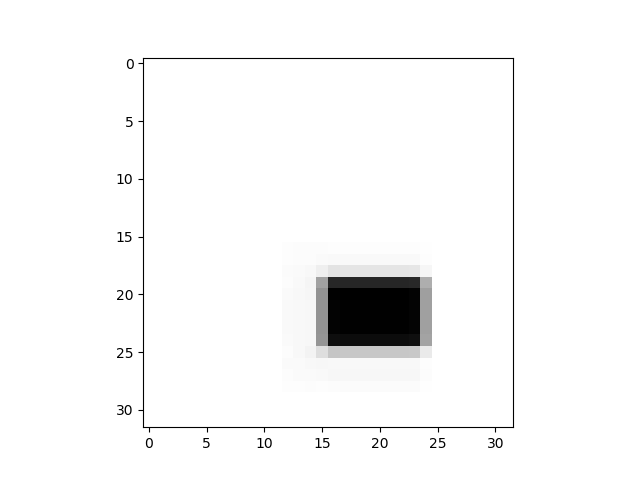
\includegraphics[width=7cm]{images/example2_0ord.png}}\\
		
		\subfloat[]{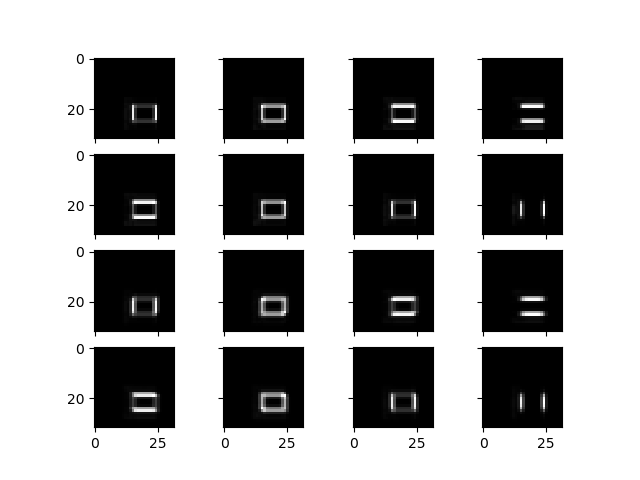
\includegraphics[width=7cm]{images/example2_1ord.png}} &
		\subfloat[]{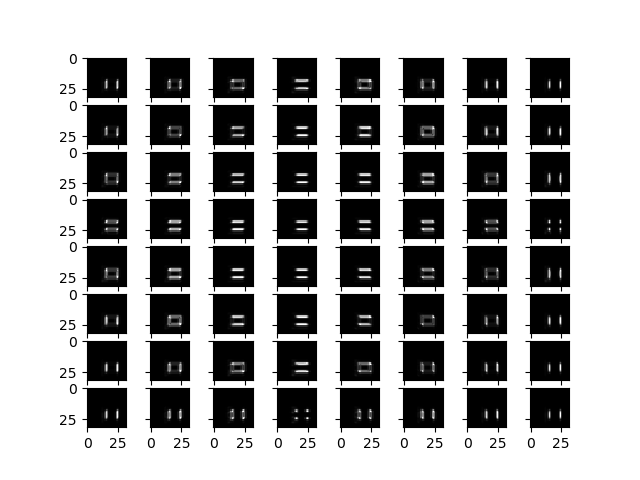
\includegraphics[width=7cm]{images/example2_2ord.png}}
	\end{tabular}
	\caption{Image taken from a toy dataset created for this work. a) Original image; b) 0th order scattering coefficients, i.e. a Gaussian low-pass filter; c) First order scattering coefficients; d) Second order scattering coefficients}
	\label{fig:example2_coefficients}
\end{figure}

%first ellipse
\begin{figure}
	\centering
	\begin{tabular}{cc}
		\subfloat[]{\fbox{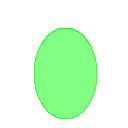
\includegraphics[width=4.5cm]{images/0000027_09.jpg}}} 
		& \subfloat[]{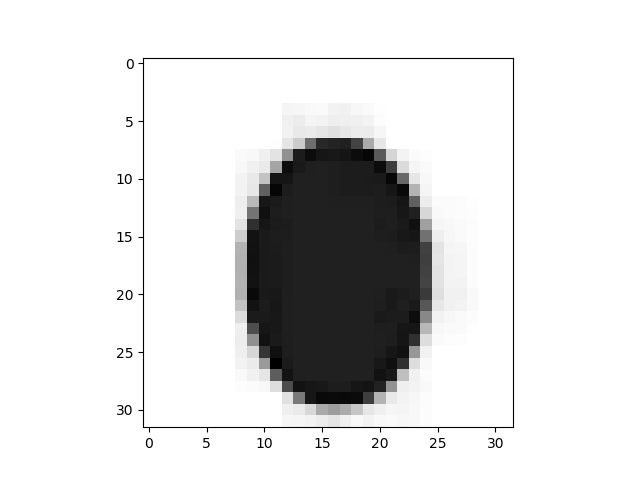
\includegraphics[width=7cm]{images/example1e_0ord.png}}\\
		
		\subfloat[]{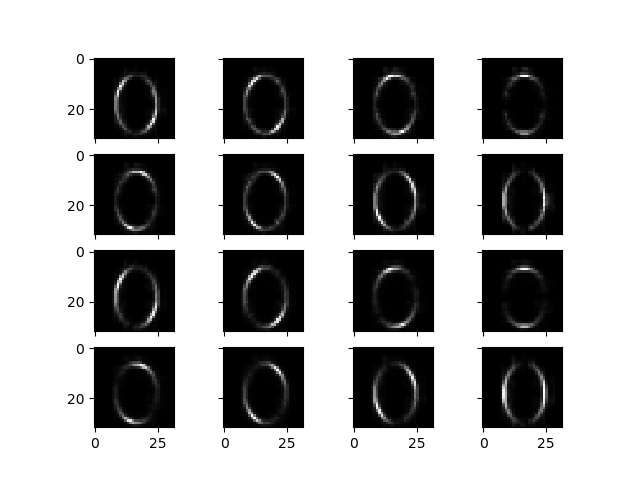
\includegraphics[width=7cm]{images/example1e_1ord.png}} &
		\subfloat[]{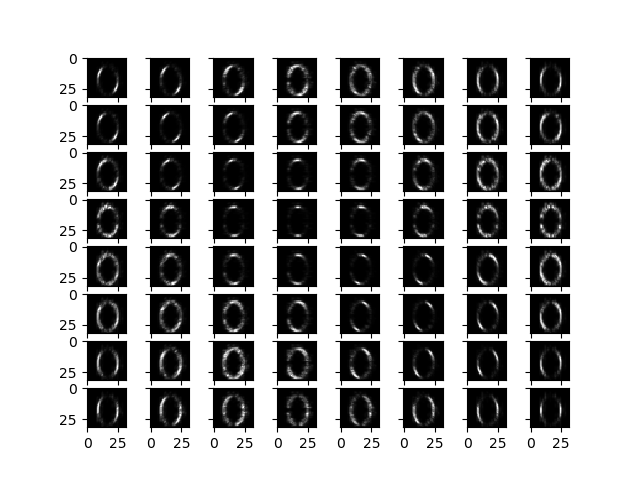
\includegraphics[width=7cm]{images/example1e_2ord.png}}
	\end{tabular}
	\caption{Image taken from a toy dataset created for this work. a) Original image; b) 0th order scattering coefficients, i.e. a Gaussian low-pass filter; c) First order scattering coefficients; d) Second order scattering coefficients}
	\label{fig:example1e_coefficients}
\end{figure}

%second ellipse
\begin{figure}
	\centering
	\begin{tabular}{cc}
		\subfloat[]{\fbox{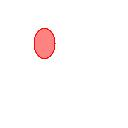
\includegraphics[width=4.5cm]{images/0000027_10.jpg}}} 
		& \subfloat[]{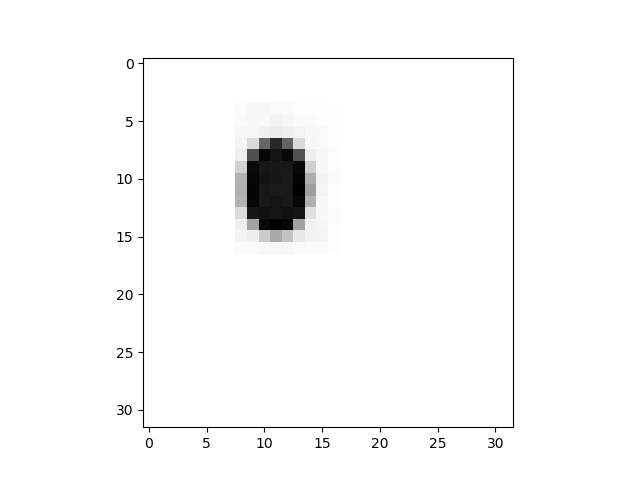
\includegraphics[width=7cm]{images/example2e_0ord.png}}\\
		
		\subfloat[]{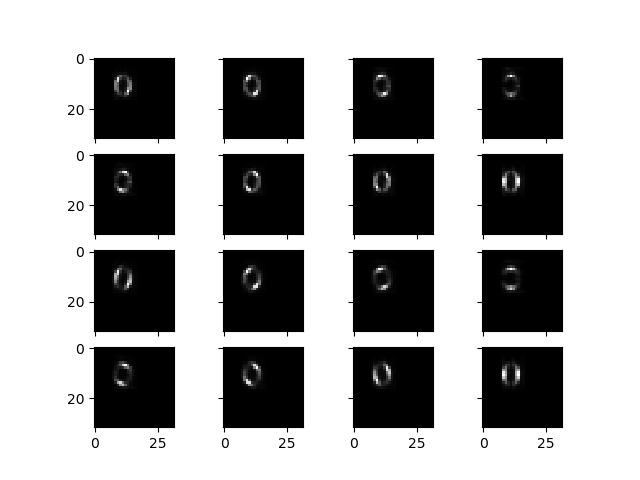
\includegraphics[width=7cm]{images/example2e_1ord.png}} &
		\subfloat[]{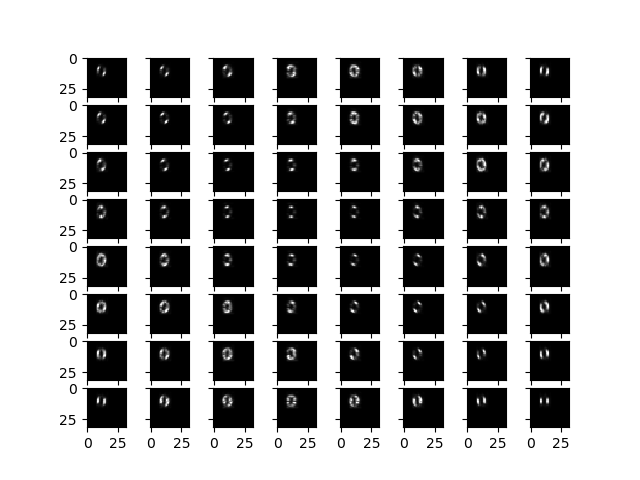
\includegraphics[width=7cm]{images/example2e_2ord.png}}
	\end{tabular}
	\caption{Image taken from a toy dataset created for this work. a) Original image; b) 0th order scattering coefficients, i.e. a Gaussian low-pass filter; c) First order scattering coefficients; d) Second order scattering coefficients}
	\label{fig:example2e_coefficients}
\end{figure}


\section{Results}

\begin{figure}[!htb]
	\centering
%	\begin{tabular}{cccc}
%		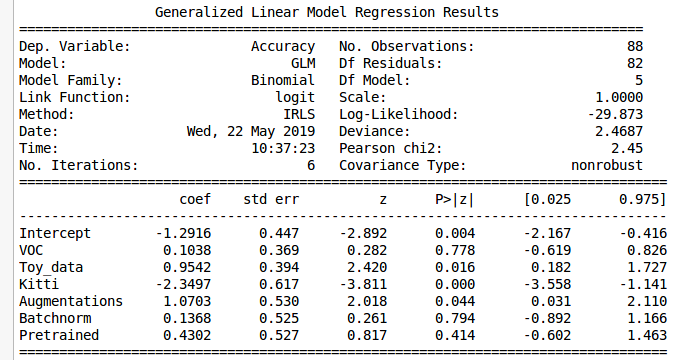
\includegraphics[width=\textwidth]{images/GLM_baselines.png}
%	\end{tabular}
	\begin{center}
		\begin{tabular}{lclc}
			\toprule
			\textbf{Dep. Variable:} &     Accuracy     & \textbf{  No. Observations:  } &       88    \\
			\textbf{Model:}         &       GLM        & \textbf{  Df Residuals:      } &       82    \\
			\textbf{Model Family:}  &     Binomial     & \textbf{  Df Model:          } &        5    \\
			\textbf{Link Function:} &      logit       & \textbf{  Scale:             } &    1.0000   \\
			\textbf{Method:}        &       IRLS       & \textbf{  Log-Likelihood:    } &   -29.873   \\
			\textbf{Date:}          & Wed, 12 Jun 2019 & \textbf{  Deviance:          } &    2.4687   \\
			\textbf{Time:}          &     16:47:27     & \textbf{  Pearson chi2:      } &     2.45    \\
			\bottomrule
		\end{tabular}
		\begin{tabular}{lcccccc}
			& \textbf{coef} & \textbf{std err} & \textbf{z} & \textbf{P$>$$|$z$|$} & \textbf{[0.025} & \textbf{0.975]}  \\
			\midrule
			\textbf{Intercept}     &      -1.2916  &        0.447     &    -2.892  &         0.004        &       -2.167    &       -0.416     \\
			\textbf{VOC}           &       0.1038  &        0.369     &     0.282  &         0.778        &       -0.619    &        0.826     \\
			\textbf{Toy\_data}     &       0.9542  &        0.394     &     2.420  &         0.016        &        0.182    &        1.727     \\
			\textbf{Kitti}         &      -2.3497  &        0.617     &    -3.811  &         0.000        &       -3.558    &       -1.141     \\
			\textbf{Augmentations} &       1.0703  &        0.530     &     2.018  &         0.044        &        0.031    &        2.110     \\
			\textbf{Batchnorm}     &       0.1368  &        0.525     &     0.261  &         0.794        &       -0.892    &        1.166     \\
			\textbf{Pretrained}    &       0.4302  &        0.527     &     0.817  &         0.414        &       -0.602    &        1.463     \\
			\bottomrule
		\end{tabular}
		%\caption{Generalized Linear Model Regression Results}
	\end{center}
	\caption{GLM for the baseline experiments. Positive coefficients imply a better accuracy. P-values below 0.05 are significant.}
	\label{fig:GLM_baseline}
\end{figure}

\begin{figure}[!htb]
	\centering
	\begin{center}
		\begin{tabular}{lclc}
			\toprule
			\textbf{Dep. Variable:}    &     Accuracy     & \textbf{  No. Observations:  } &       42    \\
			\textbf{Model:}            &       GLM        & \textbf{  Df Residuals:      } &       37    \\
			\textbf{Model Family:}     &     Binomial     & \textbf{  Df Model:          } &        4    \\
			\textbf{Link Function:}    &      logit       & \textbf{  Scale:             } &    1.0000   \\
			\textbf{Method:}           &       IRLS       & \textbf{  Log-Likelihood:    } &   -11.790   \\
			\textbf{Date:}             & Wed, 12 Jun 2019 & \textbf{  Deviance:          } &  0.086250   \\
			\textbf{Time:}             &     16:46:44     & \textbf{  Pearson chi2:      } &   0.0930    \\
			\bottomrule
		\end{tabular}
		\begin{tabular}{lcccccc}
			& \textbf{coef} & \textbf{std err} & \textbf{z} & \textbf{P$>$$|$z$|$} & \textbf{[0.025} & \textbf{0.975]}  \\
			\midrule
			\textbf{Intercept}         &      -0.5830  &        1.724     &    -0.338  &         0.735        &       -3.962    &        2.796     \\
			\textbf{Deformation\_data} &       2.9682  &        1.903     &     1.560  &         0.119        &       -0.761    &        6.697     \\
			\textbf{Rotation\_data}    &       1.1550  &        1.756     &     0.658  &         0.511        &       -2.287    &        4.597     \\
			\textbf{Scale\_data}       &       1.2074  &        1.770     &     0.682  &         0.495        &       -2.261    &        4.676     \\
			\textbf{Translation\_data} &      -5.9137  &        6.678     &    -0.886  &         0.376        &      -19.002    &        7.175     \\
			\textbf{Pretrained}        &      -0.0920  &        0.822     &    -0.112  &         0.911        &       -1.704    &        1.520     \\
			\bottomrule
		\end{tabular}
		%\caption{Generalized Linear Model Regression Results}
	\end{center}
	\caption{GLM for the baseline invariant experiments. Positive coefficients imply a better accuracy. P-values below 0.05 are significant.}
	\label{fig:GLM_invariances}
\end{figure}

\begin{figure}[!htb]
	\centering
	\begin{center}
		\begin{tabular}{lclc}
			\toprule
			\textbf{Dep. Variable:}         &     Accuracy     & \textbf{  No. Observations:  } &       36    \\
			\textbf{Model:}                 &       GLM        & \textbf{  Df Residuals:      } &       31    \\
			\textbf{Model Family:}          &     Binomial     & \textbf{  Df Model:          } &        4    \\
			\textbf{Link Function:}         &      logit       & \textbf{  Scale:             } &    1.0000   \\
			\textbf{Method:}                &       IRLS       & \textbf{  Log-Likelihood:    } &   -8.0310   \\
			\textbf{Date:}                  & Wed, 12 Jun 2019 & \textbf{  Deviance:          } &    1.3209   \\
			\textbf{Time:}                  &     16:43:30     & \textbf{  Pearson chi2:      } &     1.27    \\
			\bottomrule
		\end{tabular}
		\begin{tabular}{lcccccc}
			& \textbf{coef} & \textbf{std err} & \textbf{z} & \textbf{P$>$$|$z$|$} & \textbf{[0.025} & \textbf{0.975]}  \\
			\midrule
			\textbf{Intercept}              &      -1.0483  &        0.356     &    -2.947  &         0.003        &       -1.745    &       -0.351     \\
			\textbf{Toy\_data\_small}       &       0.6860  &        0.549     &     1.250  &         0.211        &       -0.390    &        1.762     \\
			\textbf{VOC}                    &      -1.7343  &        0.706     &    -2.457  &         0.014        &       -3.118    &       -0.351     \\
			\textbf{twentyfivek}            &       1.1156  &        0.637     &     1.751  &         0.080        &       -0.133    &        2.364     \\
			\textbf{fivek}                  &      -2.1638  &        0.881     &    -2.457  &         0.014        &       -3.890    &       -0.437     \\
			\textbf{standard}               &       0.2188  &        0.735     &     0.298  &         0.766        &       -1.222    &        1.660     \\
			\textbf{sequential\_scattering} &       0.0583  &        0.740     &     0.079  &         0.937        &       -1.392    &        1.509     \\
			\textbf{parallel\_scattering}   &      -1.3253  &        0.887     &    -1.494  &         0.135        &       -3.064    &        0.413     \\
			\bottomrule
		\end{tabular}
		%\caption{Generalized Linear Model Regression Results}
	\end{center}
	\caption{GLM for the small data experiments. Positive coefficients imply a better accuracy. P-values below 0.05 are significant.}
	\label{fig:GLM_small_data}
\end{figure}
